\documentclass[../../dissertation.tex]{subfiles}
\begin{document}

Instructions are available in the documentation for local deployment of the graphical interface.
Alternatively, users can access a web version of the app hosted online. This
version provides the same functionality as the local one and can be
accessed through a compatible web browser.\par
\begin{figure}[!h]
  \begin{minipage}{.5\linewidth}
    \centering
    \subfloat[Graph building tool]{\label{fig:gui-graph}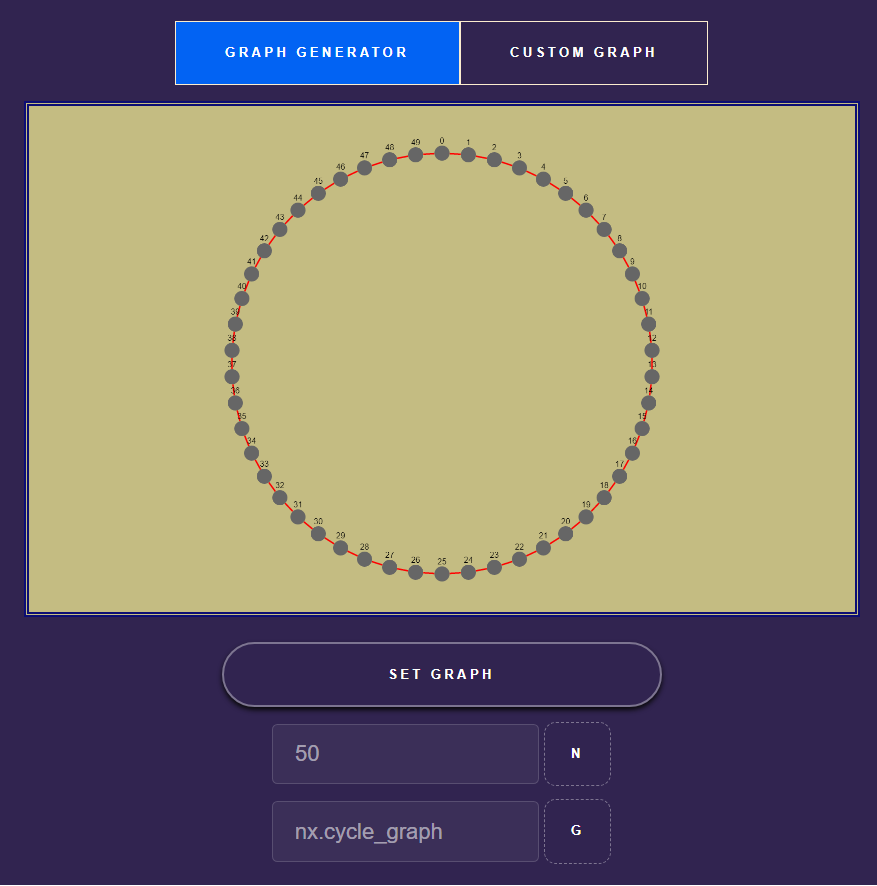
\includegraphics[scale=.25]{img/QWAK/GUI/gui-graph.png}}
  \end{minipage}%
  \begin{minipage}{.5\linewidth}
    \centering
    \subfloat[Probability distribution plot]{\label{fig:gui-probDist}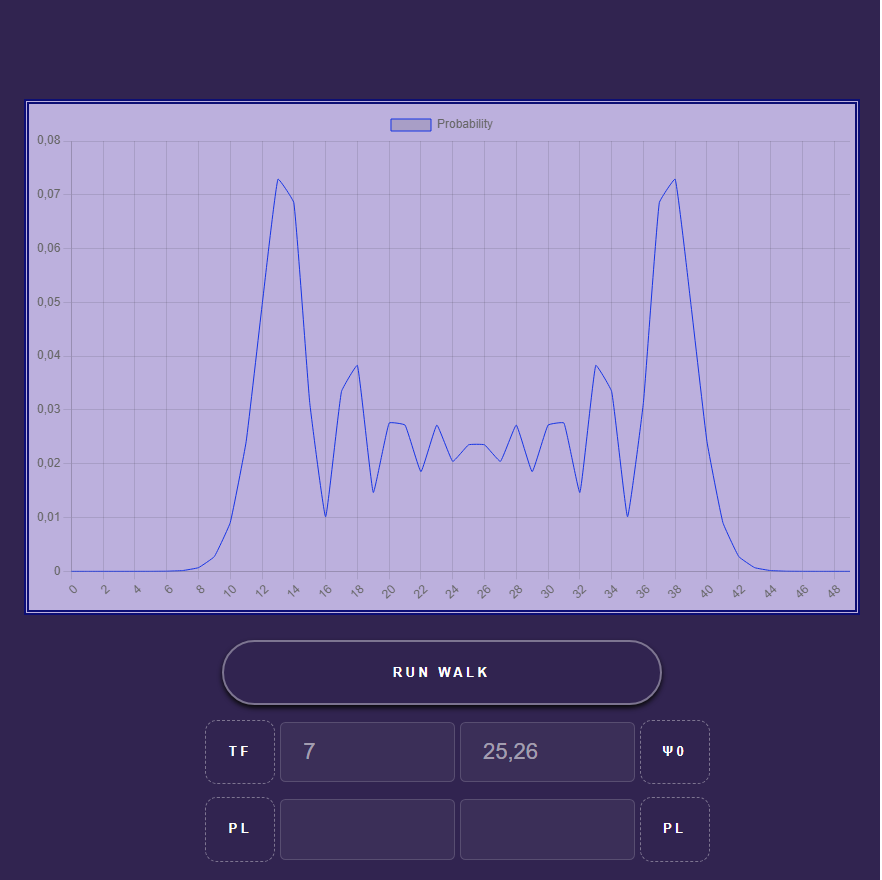
\includegraphics[scale=.25]{img/QWAK/GUI/gui-probDist.png}}
  \end{minipage}
  \caption{Main components of the graphical interface of the \texttt{QWAK} package (Part 1)}
  \label{fig:main1}
\end{figure}

The user interface offers two options for simulation: a continuous-time quantum
walk for a single instance of time, or an interval of time for dynamic
evolution. Users create graphs using the \texttt{Cytoscape} package, displayed
in figure \ref{fig:gui-graph}, either by inputting graph size and generator
name for pre-defined \texttt{NetworkX} structures, or manually through the
custom graph feature. In the future, there will be a feature for adding weights
so that directed quantum walks can be performed.\par
\begin{figure}[!h]
  \centering
  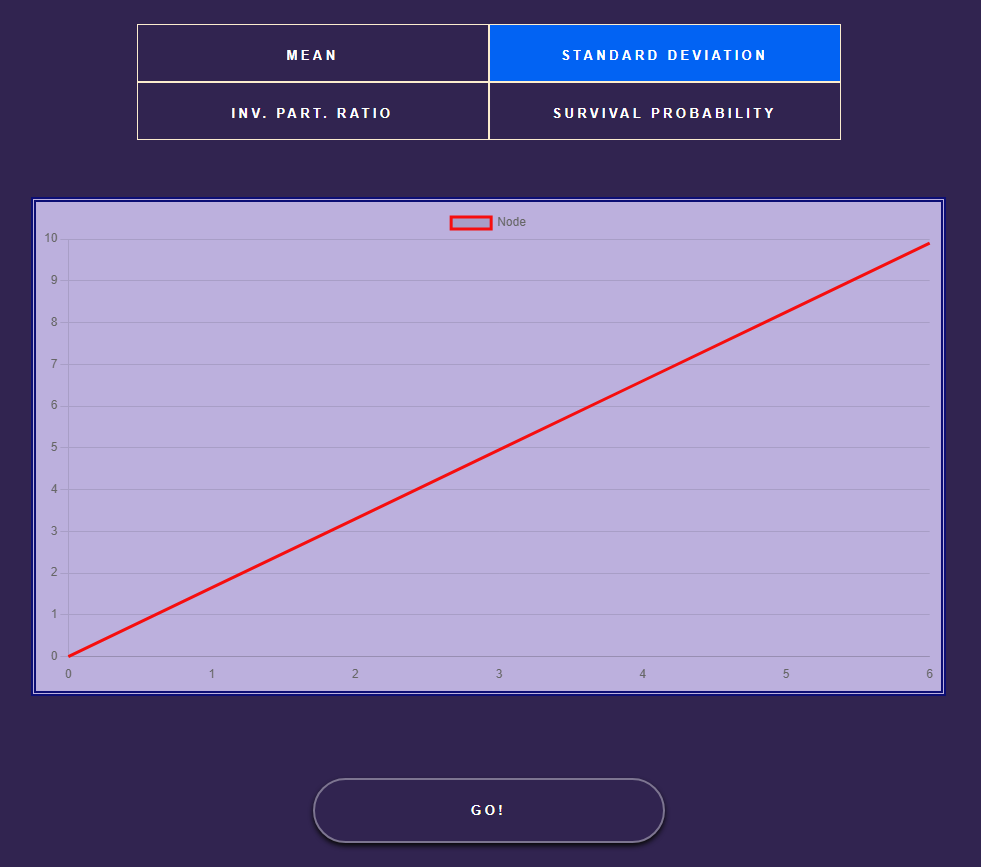
\includegraphics[scale=.25]{img/QWAK/GUI/gui-stDev.png}
  \caption{Statistical measures plot}
  \label{fig:gui-stDev}
\end{figure}

Figure \ref{fig:gui-probDist} shows the \texttt{ChartJS} object that is used to
plot the probability distributions. Users must set the initial condition and
time, currently limited to a uniform superposition state with plans to expand
to custom states. To visualize the walk dynamically, the user must specify the
lower and upper limits of the time interval. The \texttt{Flask} backend
processes this input, runs simulations via \texttt{QWAK}, and returns
JSON-formatted results, which \texttt{ChartJS} animates and displays the
evolving probability distribution.\par

In the dynamic page, the evolution of statistical measures for the quantum walk
is displayed in Figure \ref{fig:gui-stDev}, where the linear evolution of the
standard deviation is demonstrated. If the user navigates to the static page, a
table of values is provided instead. Users can specify boundary vertices for
survival probability, and transfer vertices for perfect state transfer. A
confirmation warning will appear for larger graphs, as calculating an PST can
be resource-intensive.

As future work, we plan to enhance the QWAK package with additional features,
such as support for CTQW with multiple walkers, improved visualization tools,
and integration of stochastic quantum walks into the GUI. Performance
optimizations for the \texttt{checkPST} method and the \texttt{StochasticQWAK}
class are also planned, as they are the most computationally expensive routines.

%\begin{figure}[!h]
%\begin{minipage}{.5\linewidth}
%\centering
%\subfloat[Graph building tool]{\label{fig:gui-graph}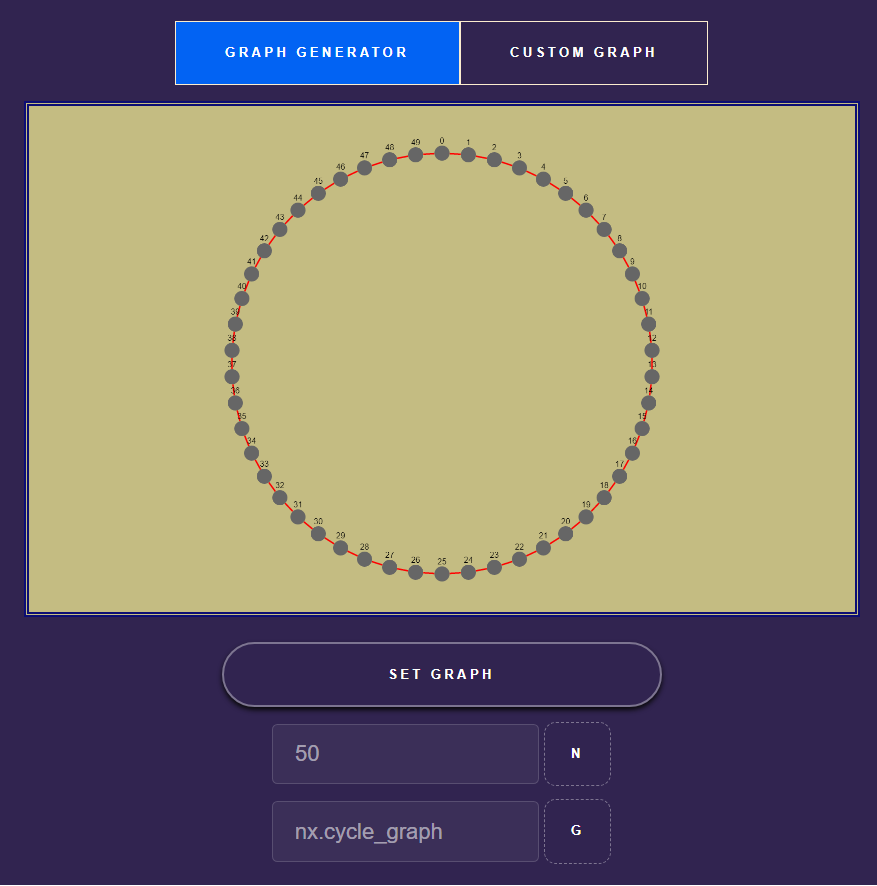
\includegraphics[scale=.25]{img/QWAK/GUI/gui-graph.png}}
%\end{minipage}%
%\begin{minipage}{.5\linewidth}
%\centering
%\subfloat[Probability distribution plot]{\label{fig:gui-probDist}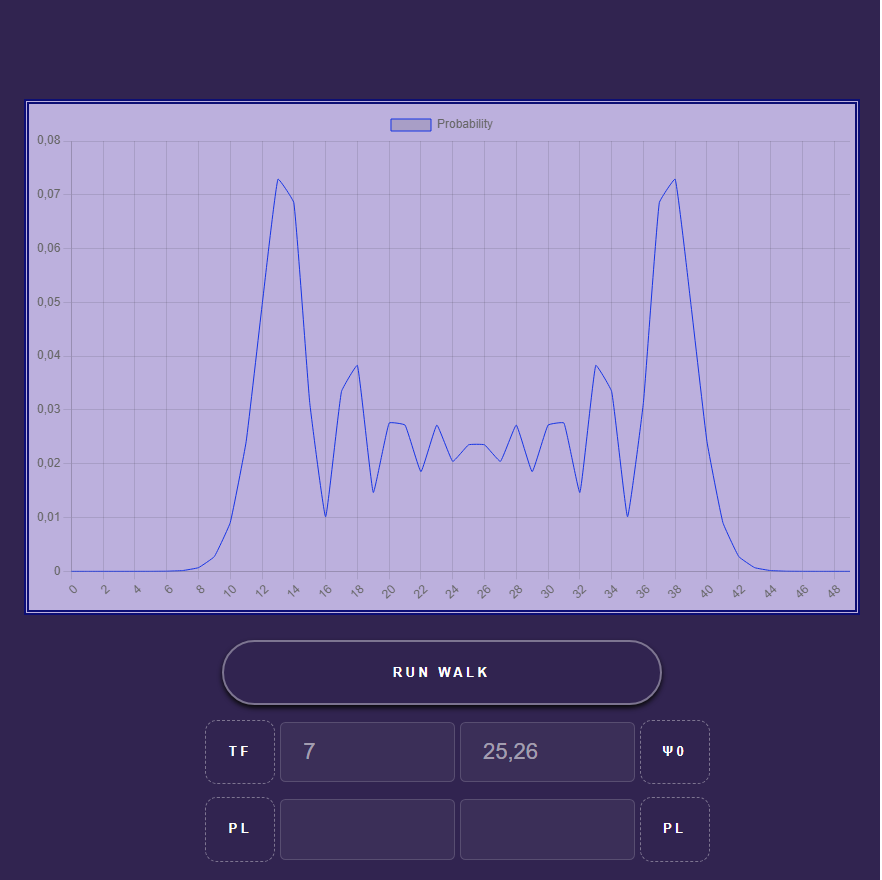
\includegraphics[scale=.25]{img/QWAK/GUI/gui-probDist.png}}
%\end{minipage}\par\medskip
%\centering
%\subfloat[Statistical measures plot]{\label{fig:gui-stDev}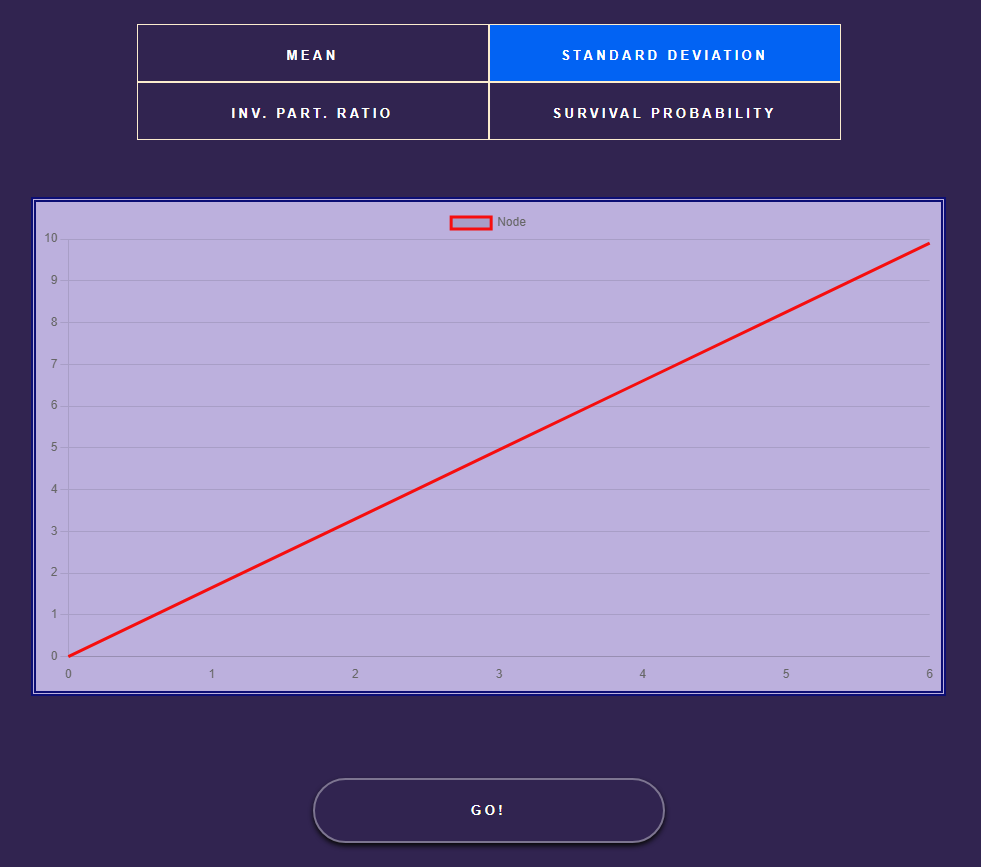
\includegraphics[scale=.25]{img/QWAK/GUI/gui-stDev.png}}
%\caption{Main components of the graphical interface of the \texttt{QWAK} package}
%\label{fig:main}
%\end{figure}
\end{document}
